\documentclass{beamer}

\usepackage{mpemath}
\usepackage{subcaption}
\usepackage[normalem]{ulem}
\usepackage{amsmath}
\usepackage{amssymb}
\usepackage{mathtools}
\usepackage{pgf}
\usepackage{pgfplots}
\usepackage{tikz}
\usepackage{booktabs}
\usepackage{siunitx}
\usepackage{natbib}
\usepackage{tabularx}
\usepackage{multirow}
\usepackage{amsmath}
\usepackage{mathtools}
\usepackage{amssymb}
\usepackage{bbm}


\usetikzlibrary{arrows,automata,backgrounds,positioning,decorations,intersections,matrix}

% *** Styles ***
\usetheme{Singapore}
\setbeamertemplate{navigation symbols}{}
% \usetheme[progressbar=frametitle]{metropolis}
% \usecolortheme{dolphin}
%\useinnertheme{circles}
%\usecolortheme{rose}
%\setbeamercovered{transparent}
\setbeamercovered{invisible}
\usefonttheme{professionalfonts}
%\usefonttheme[onlymath]{serif}
\setbeamertemplate{footline}[frame number]

\title{ROIL -- Robust Offline Imitation Learning}
\author{Gersi Doko}
\institute{Department of Computer Science \\ University of New Hampshire}
% \date{2024}

\AtBeginSection[]{
	\begin{frame}
          \vfill
	\centering
	% \usebeamerfont{title}
        {\huge\bf \insertsectionhead}%
	\vfill
\end{frame}
}

\begin{document}

\frame{\titlepage}

\section*{Intro}

\begin{frame}
	\frametitle{Robust Offline Imitation Learning}
	\textbf{Objective}: Learn a policy from expert demonstrations
	\begin{itemize}
	\item Health care: automating and improving ER care
	\item Robotics: self-driving cars, complete tasks only from demonstrations
	\item Retail: recommendation systems, customer service
	
	\end{itemize}
	\vfill
	\textbf{Offline IL}: Compute policy from a fixed dataset of expert demonstrations
	\begin{itemize}
		\item No interaction with the environment
	\end{itemize}
\end{frame}

\begin{frame}
	\frametitle{This Talk}
	Computing policies that minimize worst case regret, with respect to a possible set of experts
	\vfill
	\textbf{Outline}
	\begin{itemize}
	\item \emph{Motivation}: Why study IRL?
	\item \emph{Domain Introduction}: What is IRL?
	\item \emph{Robust Offline IL}: New approach to minimizing regret of learning from demonstrations
	\end{itemize}
\end{frame}

\section*{Motivation}

\begin{frame}
\frametitle{Motivation}
	\begin{itemize}
		\item Solve problems where it's hard to define what outcome we want
		\item Self-driving, Robotic Control, Medicine, Recommendation Systems, etc.
		\item Often have access to expert demonstrations instead of a clear description for the task
	\end{itemize}
\end{frame}

\begin{frame}
\frametitle{Motivation}
	\begin{itemize}
		\item Similar to Reinforcement Learning, but we don't have access to the true reward function $r^\star : \mathcal{S} \times \mathcal{A} \to \Real$
		\item Instead, we try and replicate the expert's behavior given their demonstrations $D_e = (s_i, \pi_e(s_i))_{i=1}^N$
		\item Generally demonstrations are given as state-action pairs collected along expert trajectories with horizon $N$
	\end{itemize}
\end{frame}

\begin{frame}
\frametitle{Motivation}
Two approaches to learning from demonstrations:
\begin{itemize}
	\item \emph{Inverse Reinforcement Learning (IRL)}: Learn a reward function from expert demonstrations then use RL to learn a policy
	\item \emph{Imitation Learning (IL)}: Learn a policy directly from expert demonstrations
\end{itemize}
	\emph{Distinction}: Inverse Reinforcement Learning (IRL) assumes problem dynamics are known, Imitation Learning (IL) does not
\end{frame}

\section*{Domain Introduction}

\begin{frame}
\frametitle{Domain Introduction}
	\begin{itemize}
		\item Our work falls into the Inverse Reinforcement Learning (IRL) category
		\item We do not attempt to learn the expert's reward function
		\item Instead, we aim to learn a policy that minimizes the regret with respect to the \emph{worst case expert} consistent with the demonstrations $D_e$
	\end{itemize}
\end{frame}

\begin{frame} \frametitle{Markov Decision Process}
  \textbf{Model} (tabular in this talk) \par
    {\small
   ~~~States $\mathcal{S}$: $s_1, s_2, s_3, \dots $ \par
   ~~~Actions $\mathcal{A}$: $a_1, a_2, \dots $ \par
   ~~~Transition probabilities $\mathcal{P} \in \Real^{\mathcal{S} \times \mathcal{A} \times \mathcal{S} }$ \par
   ~~~Initial state distribution $p_0 \in \Delta^\mathcal{S}$ \par
   ~~~Discount factor $\gamma \in \Real$ \par
   ~~~\sout{Rewards $r \in \Real^{\mathcal{S} \times \mathcal{A}}$}}
    \vfill 
    \textbf{Solution}: Policy ${\pi}\colon \mathcal{S} \to \Delta^\mathcal{A}$
    \vfill
    \textbf{Return}: Discounted expected infinite horizon return (expectation over trajectories):
    \[
	    \tilde{\rho}(\pi) = \lim_{T \to \infty} \sum_{t=0}^T \gamma^t r(\tilde{s}^{\pi}_t, \tilde{a}^{{\pi}}_t)
    \]
    \vfill
    \textbf{Random variables}: $\tilde{\rho}, \tilde{s}, \tilde{a}, \tilde{x}, \dots $ adorned with tilde
\end{frame}

\begin{frame}
	\frametitle{Domain Introduction}
\begin{itemize}
	\item We are given a dataset of state, action pairs $D_e$ generated by some expert policy $\pi_e$. \[ D_e = (s_i, \pi_e(s_i))_{i=1}^N \]
	\item $\pi_e$ follows some unknown reward function $r^\star : \mathcal{S} \times \mathcal{A} \to \Real$.
\end{itemize}
	\emph{Common assumption} : $r^\star$ can be realized by our features $\Phi : \mathcal{S} \times \mathcal{A} \to \Real^k$
	and a weight vector $w \in \mathcal{W}$ such that $r^\star = \Phi w$.

	\[ \mathcal{W} = \lbrace w \in \Real^k \mid \lvert \lvert w \rvert \rvert_1 \leq 1 \rbrace \]
\end{frame}

\section*{Our Approach}

\begin{frame}
	\frametitle{Our Approach}
	\textbf{Problem}: Find a policy $\pi$ that minimizes the regret with respect to the worst case expert consistent with the demonstrations $D_e$.
	\[ \rho(\tilde{\pi}, r) = \lim_{t \to \infty} \mathbb{E}^{\tilde{\pi}, \mathcal{P}} \lbrack \sum_{t=0}^T \gamma^t r(\tilde{s_t}, \tilde{\pi}(\tilde{s_t})) \rbrack \]
\end{frame}

\begin{frame}
	\frametitle{Our Approach}
	\textbf{Problem}: Find a policy $\pi$ that minimizes the regret with respect to the worst case expert consistent with the demonstrations $D_e$.
	\[ \rho(\tilde{\pi}, r) = \lim_{t \to \infty} \mathbb{E}^{\tilde{\pi}, \mathcal{P}} \lbrack \sum_{t=0}^T \gamma^t r(\tilde{s_t}, \tilde{\pi}(\tilde{s_t})) \rbrack \]
	\[ \Pi_R(D) = \lbrace \pi \in \Pi \mid \pi(s,a) = 1 \quad \forall (s,a) \in D \rbrace \]
\end{frame}


\begin{frame}
	\frametitle{Our Approach}
	\textbf{Problem}: Find a policy $\pi$ that minimizes the regret with respect to the worst case expert consistent with the demonstrations $D_e$.
	\[ \rho(\tilde{\pi}, r) = \lim_{t \to \infty} \mathbb{E}^{\tilde{\pi}, \mathcal{P}} \lbrack \gamma^t r(\tilde{s_t}, \tilde{\pi}(\tilde{s_t})) \rbrack \]
	\[ \Pi_R(D) = \lbrace \pi \in \Pi \mid \pi(s,a) = 1 \quad \forall (s,a) \in D \rbrace \]
	\[ \min_{\pi \in \Pi} \max_{\pi_e \in \Pi_R(D_e)} \max_{r \in \mathcal{R}} \rho(\pi_e, r) - \rho(\pi, r)\]
\end{frame}

\section*{ROIL}
\begin{frame}
	\frametitle{ROIL}
	\textbf{ROIL}: Robust Offline Imitation Learning
\[ \begin{mprog}
	\minimize{t \in \Real, u \in \Real^{\mathcal{S} \times \mathcal{A}}} t
	\stc t \geq -u\tr \Phi w + \max_{v \in \Upsilon} v\tr \Phi w,\quad \forall w \in ext(\mathcal{W}),
        \cs u\in \Upsilon,
\end{mprog} \]

Where $ext(\mathcal{W})$ is the set of extreme points of $\mathcal{W}$.

\textbf{Solution}: $u$ is the occupancy frequency of our policy, $t$ is the worst case regret.

\end{frame}

\section*{Experiments}

\begin{frame}
\frametitle{Experiments}

\begin{figure}
  \begin{center}
  \begin{minipage}{0.45\linewidth}
    \centering
    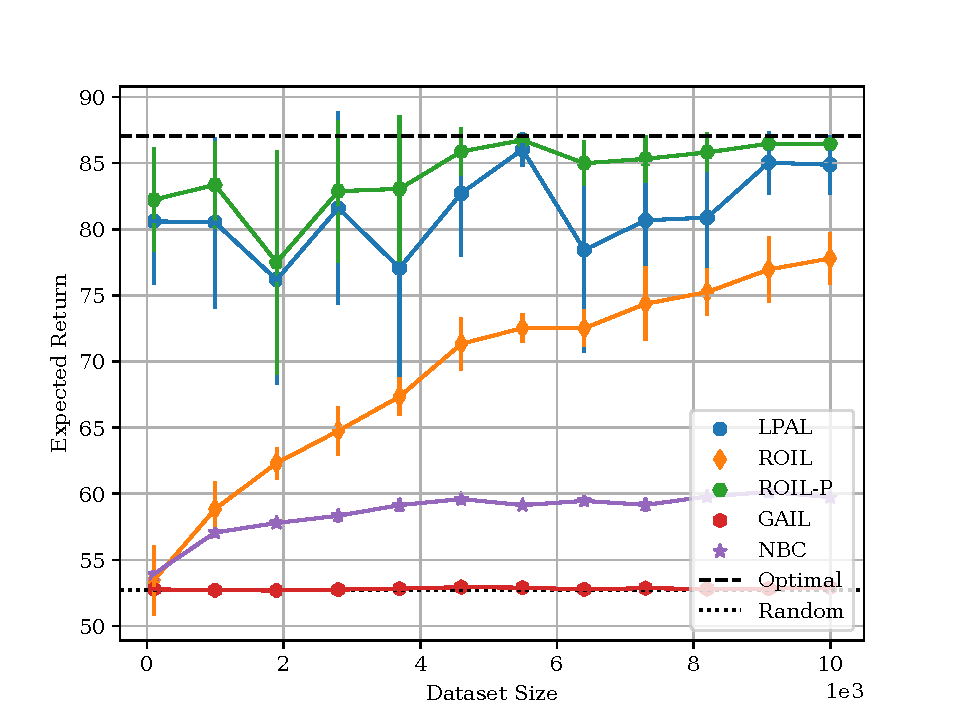
\includegraphics[width=\linewidth]{plots/returns/40x40_gridworld_on_policy_returns.pdf}
    \subcaption{On-Policy}
  \end{minipage}
  \hspace{0.05\linewidth}
  \begin{minipage}{0.45\linewidth}
    \centering
    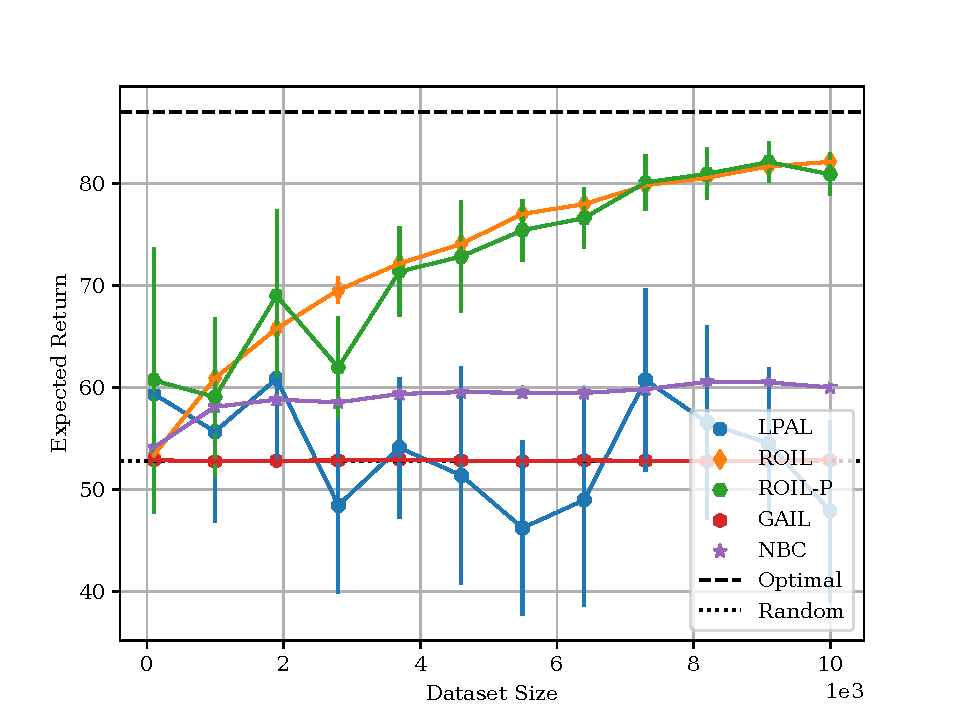
\includegraphics[width=\linewidth]{plots/returns/40x40_gridworld_off_policy_returns.pdf}
    \subcaption{Off-Policy}
  \end{minipage}
  \end{center}
\caption{Returns of ROIL and ROIL-P on 40x40 Gridworld}
\end{figure}

\end{frame}


\end{document} 
